\chapter{Statistica}
\section{Introduzione}
La distribuzione gaussiana, nota anche come distribuzione normale, è una delle più importanti distribuzioni di probabilità in statistica e nelle scienze naturali. Molte grandezze fisiche e biologiche, quando vengono misurate, tendono a seguire una distribuzione normale, soprattutto quando sono influenzate da un gran numero di piccoli effetti casuali indipendenti. Un esempio classico è l'altezza delle persone in una popolazione.

\section{Distribuzione di Probabilità}
In questa e nelle prossime sezioni, parleremo di probabilità. Quando misuriamo una grandezza casuale, vediamo che alcuni valori si ripetono più frequentemente di altri, ossia abbiamo una \textit{distribuzione} di valori. La statistica ci permette di estrarre da questa distribuzione, informazioni sulla grandezza. Si suppone che ogni grandezza abbia un valore ''vero`` e che solo effetti casuali discostino il risultato da quest'ultimo. La larghezza della distribuzione viene misurata non tanto dalla semidispersione massima (una stima troppo grande) ma dalla deviazione standard $\sigma$. Attenzione a non confonderla con l'incertezza da associare al risultato: quest'ultima è la \textit{deviazione standard della media} $\sigma_{\overline{x}} = \sigma/\sqrt{N}$, più piccola di $\sigma$ e decrescente all'aumentare del numero di misure. Ripetendo le misure molte volte, costruendo un  particolare grafico chiamato \textbf{istogramma delle frequenze}, otteniamo che questo istogramma diventa sempre  più liscio e  si avvicina ad una curva a forma di campana. In fisica, questa curva si presenta quando ripetiamo molte volte una misura casuale. In quel caso, la grandezza non ha sempre lo stesso valore ma ha, appunto, una \textit{distribuzione}. Se facciamo oscillare un pendolo, e misuriamo la durata $t$ di 20 oscillazioni con un cronometro manuale, non otterremo quasi mai due volte lo stesso valore (a causa di errori umani) ma una serie di valori. La statistica ci consente di prevedere quali saranno i valori più probabili e come questi si distribuiscono, (quanti ad esempio sono molto più grandi o più piccoli della media). Le prossime sezioni ci insegneranno come trarre informazioni utili dalla distribuzione di queste misure. Impareremo che il risultato di una misura è dato dalla media e dall'errore della media, come segue:
\[
x=\left(\overline{x} \pm \sigma_{\overline{x}}\right) \, \text{u.m.}
\]
essendo $\overline{x}$ la media dei valori e $\sigma_{\overline{x}}$ la cosiddetta deviazione standard della media.

\section{Cosa sono gli Istogrammi a Bins}
Un istogramma è uno strumento grafico utilizzato per rappresentare la distribuzione di un insieme di dati. Esso divide i dati in intervalli, chiamati \textit{bins}, e conta il numero di eventi (o frequenze) che ricadono in ciascun intervallo.

L'area di ciascun rettangolo nell'istogramma rappresenta la frequenza degli eventi nell'intervallo considerato rispetto al totale degli eventi. Questo significa che l'altezza del rettangolo (quando i bins hanno larghezze uguali) è proporzionale al numero di eventi in quel bin. Se i bins hanno larghezze diverse, l'altezza del rettangolo è proporzionale alla densità di frequenza, in modo che l'area rimanga rappresentativa della frequenza relativa.

\section{Esempio di Istogramma}

In figura \ref{fig:histogram_example} è riportato un istogramma di 1000 valori casuali estratti da una distribuzione normale, suddivisi in 30 \textit{bin}. Anche partendo da dati generati al calcolatore, si riconosce la caratteristica forma a campana, tanto più regolare quanto più numerosi sono i dati.

\begin{figure}[h!]
    \centering
    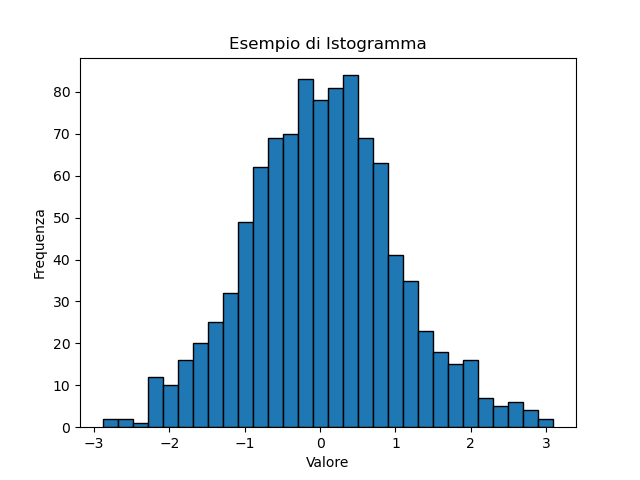
\includegraphics[width=0.8\textwidth]{img/histogram_example.png}
    \caption{Istogramma di 1000 valori con distribuzione normale, in 30 bin.}
    \label{fig:histogram_example}
\end{figure}



\section{La curva di Gauss}

La distribuzione gaussiana è caratterizzata dalla seguente funzione densità di probabilità (pdf):

\begin{equation}
f(x|\mu,\sigma) = \frac{1}{\sigma \sqrt{2\pi}} e^{-\frac{(x-\mu)^2}{2\sigma^2}}
\end{equation}

dove:
\begin{itemize}
    \item $\mu$ è la media della distribuzione, che indica il valore centrale attorno al quale i dati sono distribuiti.
    \item $\sigma$ è la deviazione standard, che misura la dispersione dei dati rispetto alla media.
\end{itemize}

La curva di Gauss ha una forma a campana, simmetrica rispetto alla media $\mu$. La maggior parte dei dati (circa il 68\%) si trova entro un intervallo di una deviazione standard dalla media ($\mu \pm \sigma$), mentre il 95\% dei dati si trova entro due deviazioni standard ($\mu \pm 2\sigma$). Questo comportamento rende la distribuzione gaussiana particolarmente utile per descrivere fenomeni naturali dove le variazioni sono dovute a molti fattori piccoli e indipendenti. In figura \ref{fig:curva_gaussiana} vediamo il tipico aspetto di una gaussiana.

\begin{figure}[h!]
    \centering
     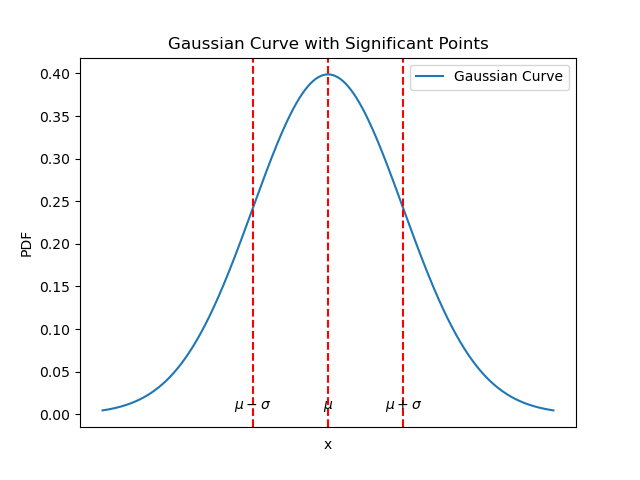
\includegraphics[scale=0.7]{img/curva_gaussiana.png} 
    \caption{Curva gaussiana con evidenziati \(\mu\), \(\mu - \sigma\) e \(\mu + \sigma\).}
    \label{fig:curva_gaussiana}
\end{figure}


\section{Esempio di istogramma sperimentale}

\subsection{Introduzione}
In questo esempio presentiamo i dati di un esperimento di misura, la fisica sottostante e il modo di costruire un istogramma che li rappresenti.

\subsection{Descrizione dell'esperimento}
L'esperimento consiste nel misurare la lunghezza di un campione di 30 barre metalliche nominalmente uguali. Le misure sono state effettuate con un calibro digitale di sensibilità $\SI{0,1}{\milli\meter}$. Di seguito sono riportati i dati sperimentali ottenuti (in cm):

\[
\begin{array}{cccccc}
45,1 & 47,2 & 49,3 & 50,5 & 52,6 & 54,7 \\
48,3 & 46,9 & 51,2 & 53,8 & 50,0 & 49,9 \\
48,7 & 51,5 & 52,1 & 47,6 & 46,3 & 50,9 \\
51,8 & 48,0 & 49,5 & 50,3 & 47,0 & 46,5 \\
52,4 & 48,8 & 49,2 & 51,3 & 47,8 & 50,7 \\
\end{array}
\]
Nei calcoli statistici useremo un foglio di calcolo e ci disinteresseremo delle cifre significative durante i passaggi intermedi; queste torneranno importanti solo quando scriveremo il risultato finale della misura.
\subsection{Fisica dell'esperimento}
La misura della lunghezza delle barre metalliche è un esperimento comune in fisica per studiare le proprietà dei materiali. La lunghezza può variare a causa di fattori come:
\begin{itemize}
    \item Differenze nel processo di produzione.
    \item Espansione termica a diverse temperature.
    \item Errori sistematici e casuali durante la misurazione.
\end{itemize}
L'istogramma delle misure permette di visualizzare la distribuzione delle lunghezze e di identificare eventuali deviazioni significative dalla media.

\subsection{Costruzione dell'istogramma}
Per costruire l'istogramma si divide l'intervallo dei dati (da circa $\SI{45}{cm}$ a circa $\SI{55}{cm}$) in un certo numero di classi di uguale ampiezza (\textit{bin}), qui 8, e si conta quante misure cadono in ciascuna classe. Il risultato è in figura \ref{fig:istogramma2}. Con un foglio di calcolo si ottiene lo stesso grafico usando la funzione \texttt{FREQUENZA} (o lo strumento ``Istogramma'') e poi un grafico a barre.

\subsection{Risultati}
L'istogramma mostra la distribuzione delle lunghezze delle barre: i valori si addensano attorno a circa $\SI{49}{cm}$--$\SI{50}{cm}$ e diventano via via più rari allontanandosi da questo intervallo. Permette anche di individuare a colpo d'occhio la variabilità delle misure e la presenza di eventuali valori anomali.

\begin{figure}[!htbp] 
    \centering
    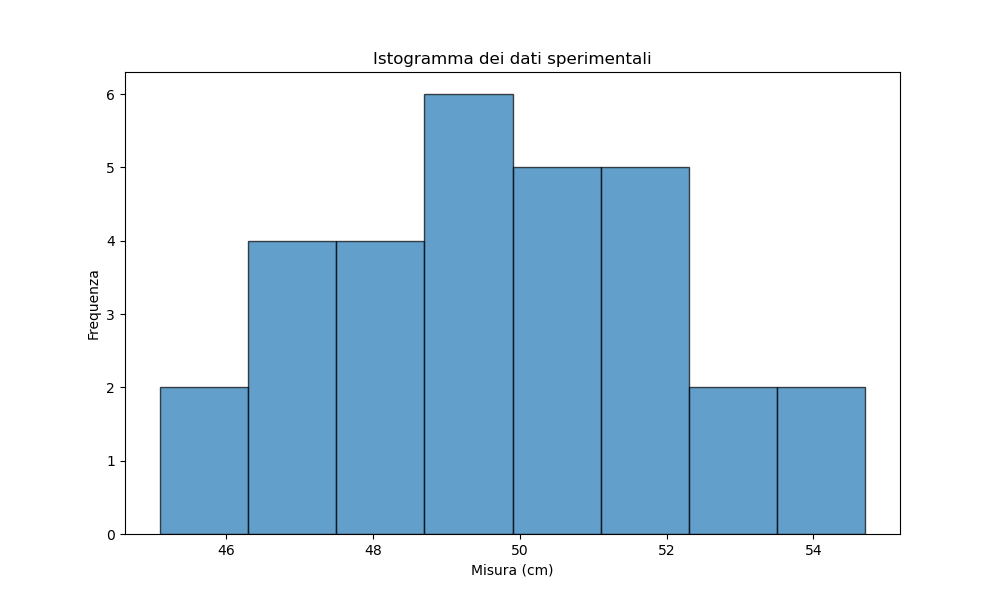
\includegraphics[width=0.8\textwidth]{img/istogramma2.png}
    \caption{Istogramma dei dati sperimentali}
    \label{fig:istogramma2}
\end{figure}



\section{Approssimazione della Gaussiana}
In un esperimento, se ripetiamo molte volte una misura e calcoliamo la media e la deviazione standard, al crescere del numero di misure l'istogramma dei dati approssima sempre meglio una distribuzione gaussiana. Ci sono due fatti distinti dietro questa osservazione. Il primo è la \textit{legge dei grandi numeri}: al crescere del numero di misure, la media e la deviazione standard calcolate coi dati si avvicinano ai loro valori ``veri'' (quelli che otterremmo con infinite misure). Il secondo è il \textit{teorema centrale del limite}: quando una grandezza è il risultato di molti piccoli effetti casuali indipendenti, la sua distribuzione tende alla forma a campana, indipendentemente da come sono fatti i singoli effetti.

Quando una persona esegue una misura, a quella persona e a quell'apparato corrisponde una certa distribuzione: i valori si sparpagliano attorno alla media in un modo che dipende dalla precisione del sistema di misura. Ad esempio, se Marco lascia cadere una pallina mille volte (povero Marco\dots) e misura i tempi di caduta con un cronometro a mano, magari otterrà una media di $\SI{0,45}{s}$ con una deviazione standard di $\SI{0,08}{s}$. Se ripetiamo l'esperimento usando una fotocellula, le misure si sparpagliano di meno: stessa media (circa $\SI{0,45}{s}$) ma deviazione standard di appena $\SI{0,01}{s}$. La grandezza da misurare (il tempo di caduta) è la stessa, ma il secondo sistema è più preciso. Costruendo gli istogrammi sperimentali, quello della misura a mano avrebbe una campana più larga, perché la deviazione standard misura proprio quanto è largo l'istogramma. 

\section{Stima di Media e Deviazione Standard}
Data una serie di $n$ misurazioni sperimentali $\{x_1, x_2, \ldots, x_n\}$, possiamo stimare i parametri della distribuzione gaussiana, cioè la media $\mu$ e la deviazione standard $\sigma$, utilizzando le seguenti formule:

\subsection{Calcolo della Media}
La media campionaria $\hat{\mu}$ è data dalla somma di tutte le osservazioni divisa per il numero totale di osservazioni:

\begin{equation}
\hat{\mu} = \frac{1}{n} \sum_{i=1}^{n} x_i
\end{equation}

\subsection{Calcolo della Deviazione Standard}
La deviazione standard campionaria $\hat{\sigma}$ è data dalla radice quadrata della somma dei quadrati delle differenze tra ciascuna osservazione e la media campionaria, divisa per il numero di osservazioni meno uno:

\begin{equation}
\hat{\sigma} = \sqrt{\frac{1}{n-1} \sum_{i=1}^{n} (x_i - \hat{\mu})^2}
\end{equation}

\subsection{Calcolo della Deviazione Standard della Media}
La deviazione standard della media, nota anche come errore standard della media, è calcolata come:

\begin{equation}
\sigma_{\overline{x}} = \frac{\hat{\sigma}}{\sqrt{n}}
\end{equation}

Dove $\hat{\sigma}$ è la deviazione standard campionaria e $n$ è il numero di osservazioni. La deviazione standard della media rappresenta quanto la media campionaria è attesa essere distante dalla media vera della popolazione. Per una stima più precisa, questa deviazione standard della media viene approssimata a una cifra significativa.

\section{Esempio pratico: le altezze di un gruppo di persone}
Per illustrare questi concetti consideriamo un insieme di 100 valori di altezza (in cm), \emph{generati al calcolatore} a partire da una distribuzione a campana (i numeri non provengono da persone reali e la larghezza è volutamente esagerata per rendere ben visibile l'effetto). Su questi dati calcoliamo media, deviazione standard e deviazione standard della media, e ne costruiamo l'istogramma con sovrapposta la curva di Gauss corrispondente.

Un foglio di calcolo (o un qualunque software di analisi dati) fornisce:
\begin{center}
\begin{tabular}{ll}
\toprule
Media delle altezze & $\overline{x} \approx \SI{167,83}{\centi\meter}$ \\
Deviazione standard & $\sigma \approx \SI{15,80}{\centi\meter}$ \\
Deviazione standard della media & $\sigma_{\overline{x}} = \sigma/\sqrt{100} \approx \SI{1,6}{\centi\meter}$ \\
\bottomrule
\end{tabular}
\end{center}
Il risultato, scritto in forma corretta (errore a una cifra significativa), è
\[
x = \left(168 \pm 2\right)\si{\centi\meter}.
\]

Nel grafico \ref{fig:istogramma} vediamo l'istogramma dei dati con sovrapposta la curva che lo approssima. In ascissa ci sono gli intervalli di altezza; in ordinata un valore tale che l'\emph{area} di ogni barra sia uguale alla frazione di persone con altezza compresa tra i suoi estremi. Ad esempio, se una barra larga da $\SI{160}{cm}$ a $\SI{172}{cm}$ ha altezza $0,025$, allora $\left(172-160\right)\times 0,025 = 0,3$: il 30\% delle persone ha altezza in quell'intervallo.

La curva è centrata sulla media ($\SI{167,83}{\centi\meter}$), indicata dalla linea rossa tratteggiata. Le due linee blu tratteggiate sono a distanza $\sigma$ dalla media: quella di destra si trova a $\SI{167,83}{\centi\meter} + \SI{15,80}{\centi\meter} = \SI{183,63}{\centi\meter}$, quella di sinistra a $\SI{152,03}{\centi\meter}$. Per una distribuzione a campana, l'area sotto la curva compresa tra le due linee blu è circa $0,68$: cioè circa il 68\% delle misure cade tra $\overline{x} - \sigma$ e $\overline{x} + \sigma$.

\begin{figure}[h!]
    \centering
    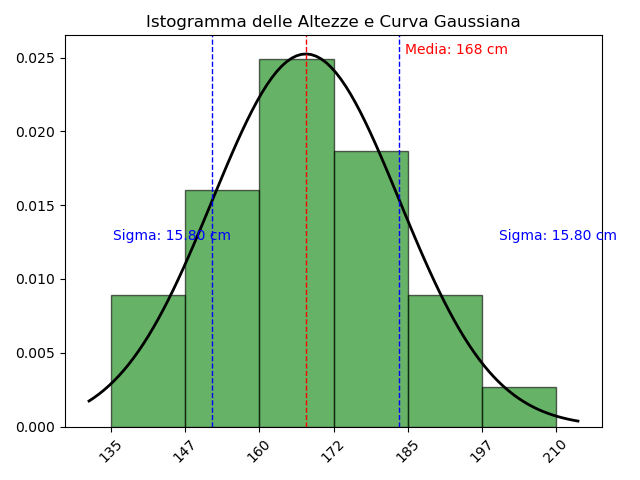
\includegraphics[width=0.8\textwidth]{img/istogramma.png}
    \caption{Istogramma delle altezze con sovrapposta la curva gaussiana. Linea rossa: media; linee blu: media $\pm\,\sigma$.}
    \label{fig:istogramma}
\end{figure}


\section{Regressione Lineare}
In fisica, il moto uniforme è un tipo di moto in cui un oggetto si sposta con velocità costante. Questo significa che la distanza percorsa dall'oggetto è proporzionale al tempo impiegato. La relazione tra spazio \( y \) e tempo \( x \) in un moto uniforme può essere espressa tramite la seguente equazione lineare:

\[
y = v \cdot x + s_0
\]

dove:
\begin{itemize}
    \item \( v \) è la velocità costante dell'oggetto (pendenza della retta).
    \item \( s_0 \) è la posizione iniziale dell'oggetto (intercetta della retta).
\end{itemize}

L'obiettivo è trovare i parametri \( v \) e \( s_0 \) che meglio rappresentano i dati sperimentali. Utilizzando una regressione lineare, possiamo ottenere questi parametri adattando una retta ai dati.

\subsection{Tabella dei Dati}

Per l'analisi, consideriamo i seguenti dati sperimentali raccolti per tempo e spazio:

\begin{table}[h!]
    \centering
    \begin{tabular}{|c|c|}
    \hline
    \textbf{Tempo (\si{\second})} & \textbf{Spazio (\si{\meter})} \\
    \hline
    1,0 & 2,1 \\
    2,0 & 3,9 \\
    3,0 & 6,2 \\
    4,0 & 7,8 \\
    5,0 & 10,1 \\
    \hline
    \end{tabular}
    \caption{Dati sperimentali di tempo e spazio.}
    \label{tab:dati}
\end{table}

\subsection{Regressione Lineare}

La regressione lineare cerca di adattare una retta ai dati sperimentali, trovando i parametri \( a \) e \( b \) che minimizzano la somma dei quadrati delle differenze tra i valori osservati e quelli previsti dalla retta. In questo caso, la retta di regressione è data da:

\[
y = a \cdot x + b
\]

dove:
\begin{itemize}
    \item \( a \) è la pendenza della retta, che rappresenta la velocità \( v \).
    \item \( b \) è l'intercetta, che rappresenta la posizione iniziale \( s_0 \).
\end{itemize}

\subsection{Calcolo della retta di regressione}
Tutti i fogli di calcolo hanno funzioni dedicate per la regressione lineare (ad esempio \texttt{PENDENZA} e \texttt{INTERCETTA}, oppure lo strumento ``linea di tendenza'' sul grafico a dispersione, che può mostrare direttamente l'equazione della retta). Applicandole ai dati della tabella \ref{tab:dati} si ottiene:

\begin{mdframed}[backgroundcolor=lightgray, linecolor=black, linewidth=1pt]
\textbf{Pendenza} $a$: \(\left(1,99 \pm 0,06\right) \, \si{\meter\per\second}\) \\
\textbf{Intercetta} $b$: \(\left(0,05 \pm 0,20\right) \, \si{\meter}\)
\end{mdframed}

\textbf{Pendenza}: rappresenta la velocità media del moto. L'errore associato indica di quanto la pendenza è incerta, e riflette la dispersione dei dati sperimentali attorno alla retta.

\textbf{Intercetta}: rappresenta la posizione iniziale $s_0$, cioè il valore di $y$ quando $x = 0$. Qui è compatibile con zero entro l'errore, coerente con un moto che parte dall'origine.

Di seguito, in figura \ref{fig:regressione_lineare} è mostrato il grafico della regressione lineare, con i dati sperimentali e la retta ottenuta.

\begin{figure}[h!]
    \centering
    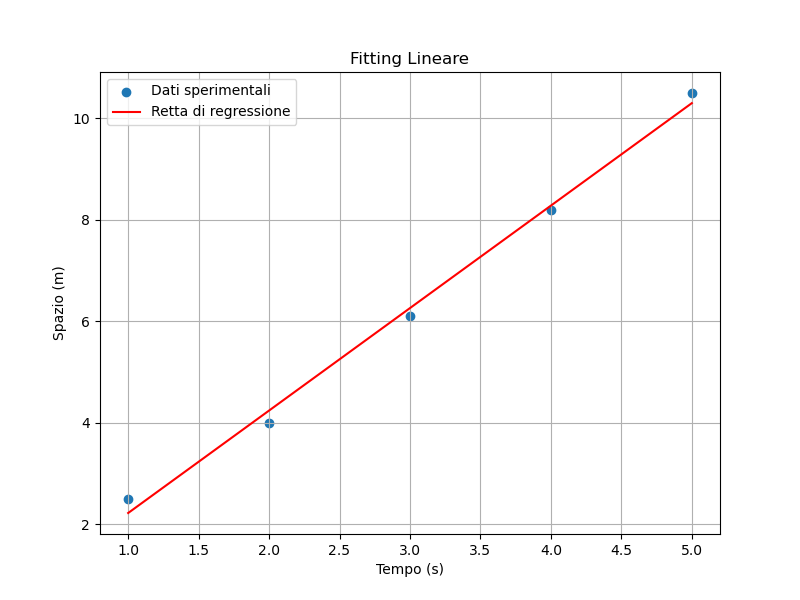
\includegraphics[width=0.8\textwidth]{img/regressione_lineare.png}
    \caption{Grafico della regressione lineare: i dati sperimentali sono mostrati come punti, e la retta di regressione è mostrata in rosso.}
    \label{fig:regressione_lineare}
\end{figure}


\section{Esempio complesso: misura di \texorpdfstring{$g$}{g} da un moto di caduta}
Supponiamo di avere i dati sperimentali nella tabella \ref{tab:regrcompl}, che riportano la distanza percorsa in caduta libera in funzione del tempo:
\begin{table}[h!]
\centering
\begin{tabular}{|c|c|}
\hline
Tempo (s) & Distanza (m) \\
\hline
1,0 & 4,9 \\
2,0 & 19,6 \\
3,0 & 44,1 \\
4,0 & 78,4 \\
5,0 & 122,5 \\
\hline
\end{tabular}
\caption{Dati di un moto di caduta.}
\label{tab:regrcompl}
\end{table}

\subsection{Linearizzazione}
La relazione tra distanza e tempo nella caduta libera è
\[
s=\frac{1}{2}\,g\,t^2 ,
\]
cioè una relazione \emph{quadratica} tra $s$ e $t$. Se però introduciamo la nuova variabile $u = t^2$, la relazione diventa \emph{lineare}:
\[
s=\frac{1}{2}\,g\,u = b\cdot u , \qquad b=\frac{g}{2},
\]
ed è una retta \emph{passante per l'origine} (nessuna intercetta). Costruiamo quindi la colonna dei valori di $u = t^2$:
\begin{center}
\begin{tabular}{|c|c|}
\hline
Tempo $t$ (s) & $u = t^2$ (s$^2$) \\
\hline
1,0 & 1,0 \\
2,0 & 4,0 \\
3,0 & 9,0 \\
4,0 & 16,0 \\
5,0 & 25,0 \\
\hline
\end{tabular}
\end{center}
Riportiamo $s$ in funzione di $u$ su un grafico a dispersione e tracciamo la linea di tendenza lineare \emph{con intercetta fissata a zero}. Il foglio di calcolo fornisce la pendenza $b$ e (con lo strumento di regressione) il suo errore $\sigma_b$. Una volta trovato $b$, l'accelerazione di gravità e il suo errore si ricavano con:
\[
g = 2\,b , \qquad \sigma_g = 2\,\sigma_b .
\]

\subsection{Risultato}
Il grafico è mostrato in figura \ref{fig:g}. Dalla pendenza della retta si ottiene:
\[
g = \left(9,80 \pm 0,01\right)\si{\meter\per\square\second},
\]
in ottimo accordo con il valore noto $g \approx \SI{9,81}{\meter\per\square\second}$.

\begin{figure}[!htbp]
    \centering
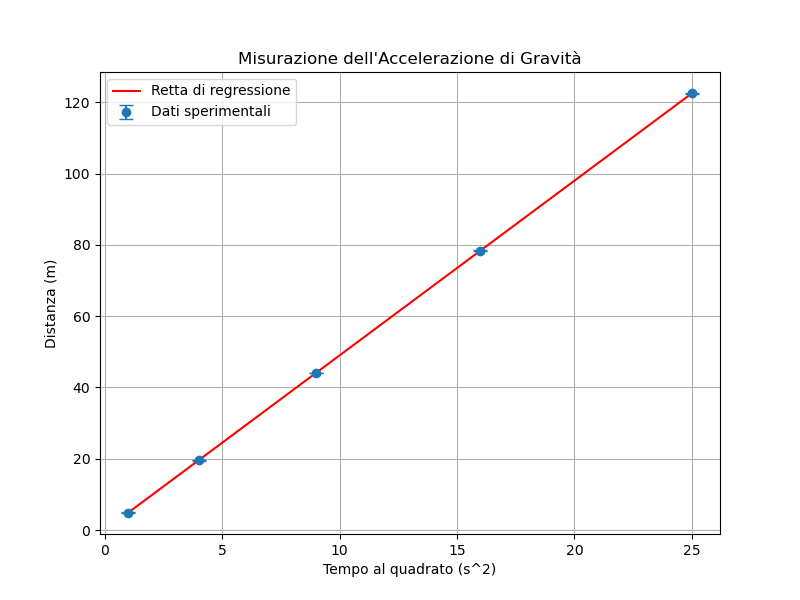
\includegraphics[scale=0.6]{img/g.png}
    \caption{Grafico di $s$ in funzione di $t^2$: la pendenza della retta vale $g/2$.}
    \label{fig:g}
\end{figure}

\section{Conclusioni}

In questo capitolo abbiamo introdotto due strumenti fondamentali per l'analisi dei dati sperimentali: le distribuzioni di probabilità (con la distribuzione gaussiana e gli istogrammi) e la regressione lineare.

\subsection{Distribuzioni di probabilità e istogrammi}
Le distribuzioni di probabilità descrivono come si distribuiscono i valori di una grandezza soggetta a effetti casuali. L'istogramma è lo strumento visivo per rappresentarle: l'area di ogni barra è proporzionale alla frazione di dati che cade nel corrispondente intervallo. Quando una grandezza è il risultato di molti piccoli effetti casuali indipendenti, la sua distribuzione tende alla forma a campana (gaussiana), caratterizzata da media $\mu$ e deviazione standard $\sigma$; circa il 68\% dei dati cade tra $\mu-\sigma$ e $\mu+\sigma$.

\subsection{Regressione lineare}
La regressione lineare cerca la retta $y = a x + b$ che meglio approssima una serie di dati, minimizzando la somma dei quadrati degli scarti. È particolarmente utile in fisica perché molte leggi, anche non lineari, si possono ricondurre a una relazione lineare con un opportuno cambio di variabile (linearizzazione), come nella misura di $g$ dalla caduta di un grave. Pendenza e intercetta, con i loro errori, si ottengono direttamente dagli strumenti di regressione dei fogli di calcolo.



